\documentclass[11pt,a4paper]{article}
\usepackage[utf8]{inputenc}
\usepackage{amsmath,amsfonts,amssymb}
\usepackage{graphicx}
\usepackage{geometry}
\geometry{margin=1in}
\usepackage{booktabs}
\usepackage{hyperref}
\usepackage{float}
\usepackage{xcolor}

\definecolor{darkbg}{HTML}{0d121f}
\definecolor{lighttext}{HTML}{e2e8f0}
\definecolor{primary}{HTML}{8b5cf6}
\definecolor{secondary}{HTML}{0dd5c5}

\pagecolor{darkbg}
\color{lighttext}

\hypersetup{
    colorlinks=true,
    linkcolor=secondary,
    urlcolor=secondary
}

\title{\textbf{EE3621: Digital Signal Processing} \\ \Large Lecture 30: DSP Capstone --- System Design, Implementation \& Future Trends \\ \large (III B.Tech EEE)}
\author{Lecture Notes (40-Minute Plan)}
\date{}

\begin{document}

\maketitle

\section{Lecture Plan (40 Minutes Breakdown)}
\begin{itemize}
    \item \textbf{00:00 -- 05:00 (5 mins):} System Design Methodology: Requirements, algorithmic choices, fixed vs floating point.
    \item \textbf{05:00 -- 12:00 (7 mins):} Fixed-Point DSP Implementation: Q-format notation, overflow, scaling, and rounding strategies.
    \item \textbf{12:00 -- 18:00 (6 mins):} DSP Processor Architecture: Harvard architecture, MAC, barrel shifter, circular buffers, and SIMD.
    \item \textbf{18:00 -- 22:00 (4 mins):} Hardware Trade-offs (FPGA vs DSP vs GPU) \& Real-Time System Design.
    \item \textbf{22:00 -- 30:00 (8 mins):} Course Review: Interconnections of key topics.
    \item \textbf{30:00 -- 35:00 (5 mins):} Emerging Trends (TinyML, QSP) \& Career Paths in DSP.
    \item \textbf{35:00 -- 40:00 (5 mins):} Comprehensive Final Exam Problems discussion.
\end{itemize}

\noindent\rule{\textwidth}{0.5pt}

\section{System Design Methodology}

\begin{figure}[H]
    \centering
    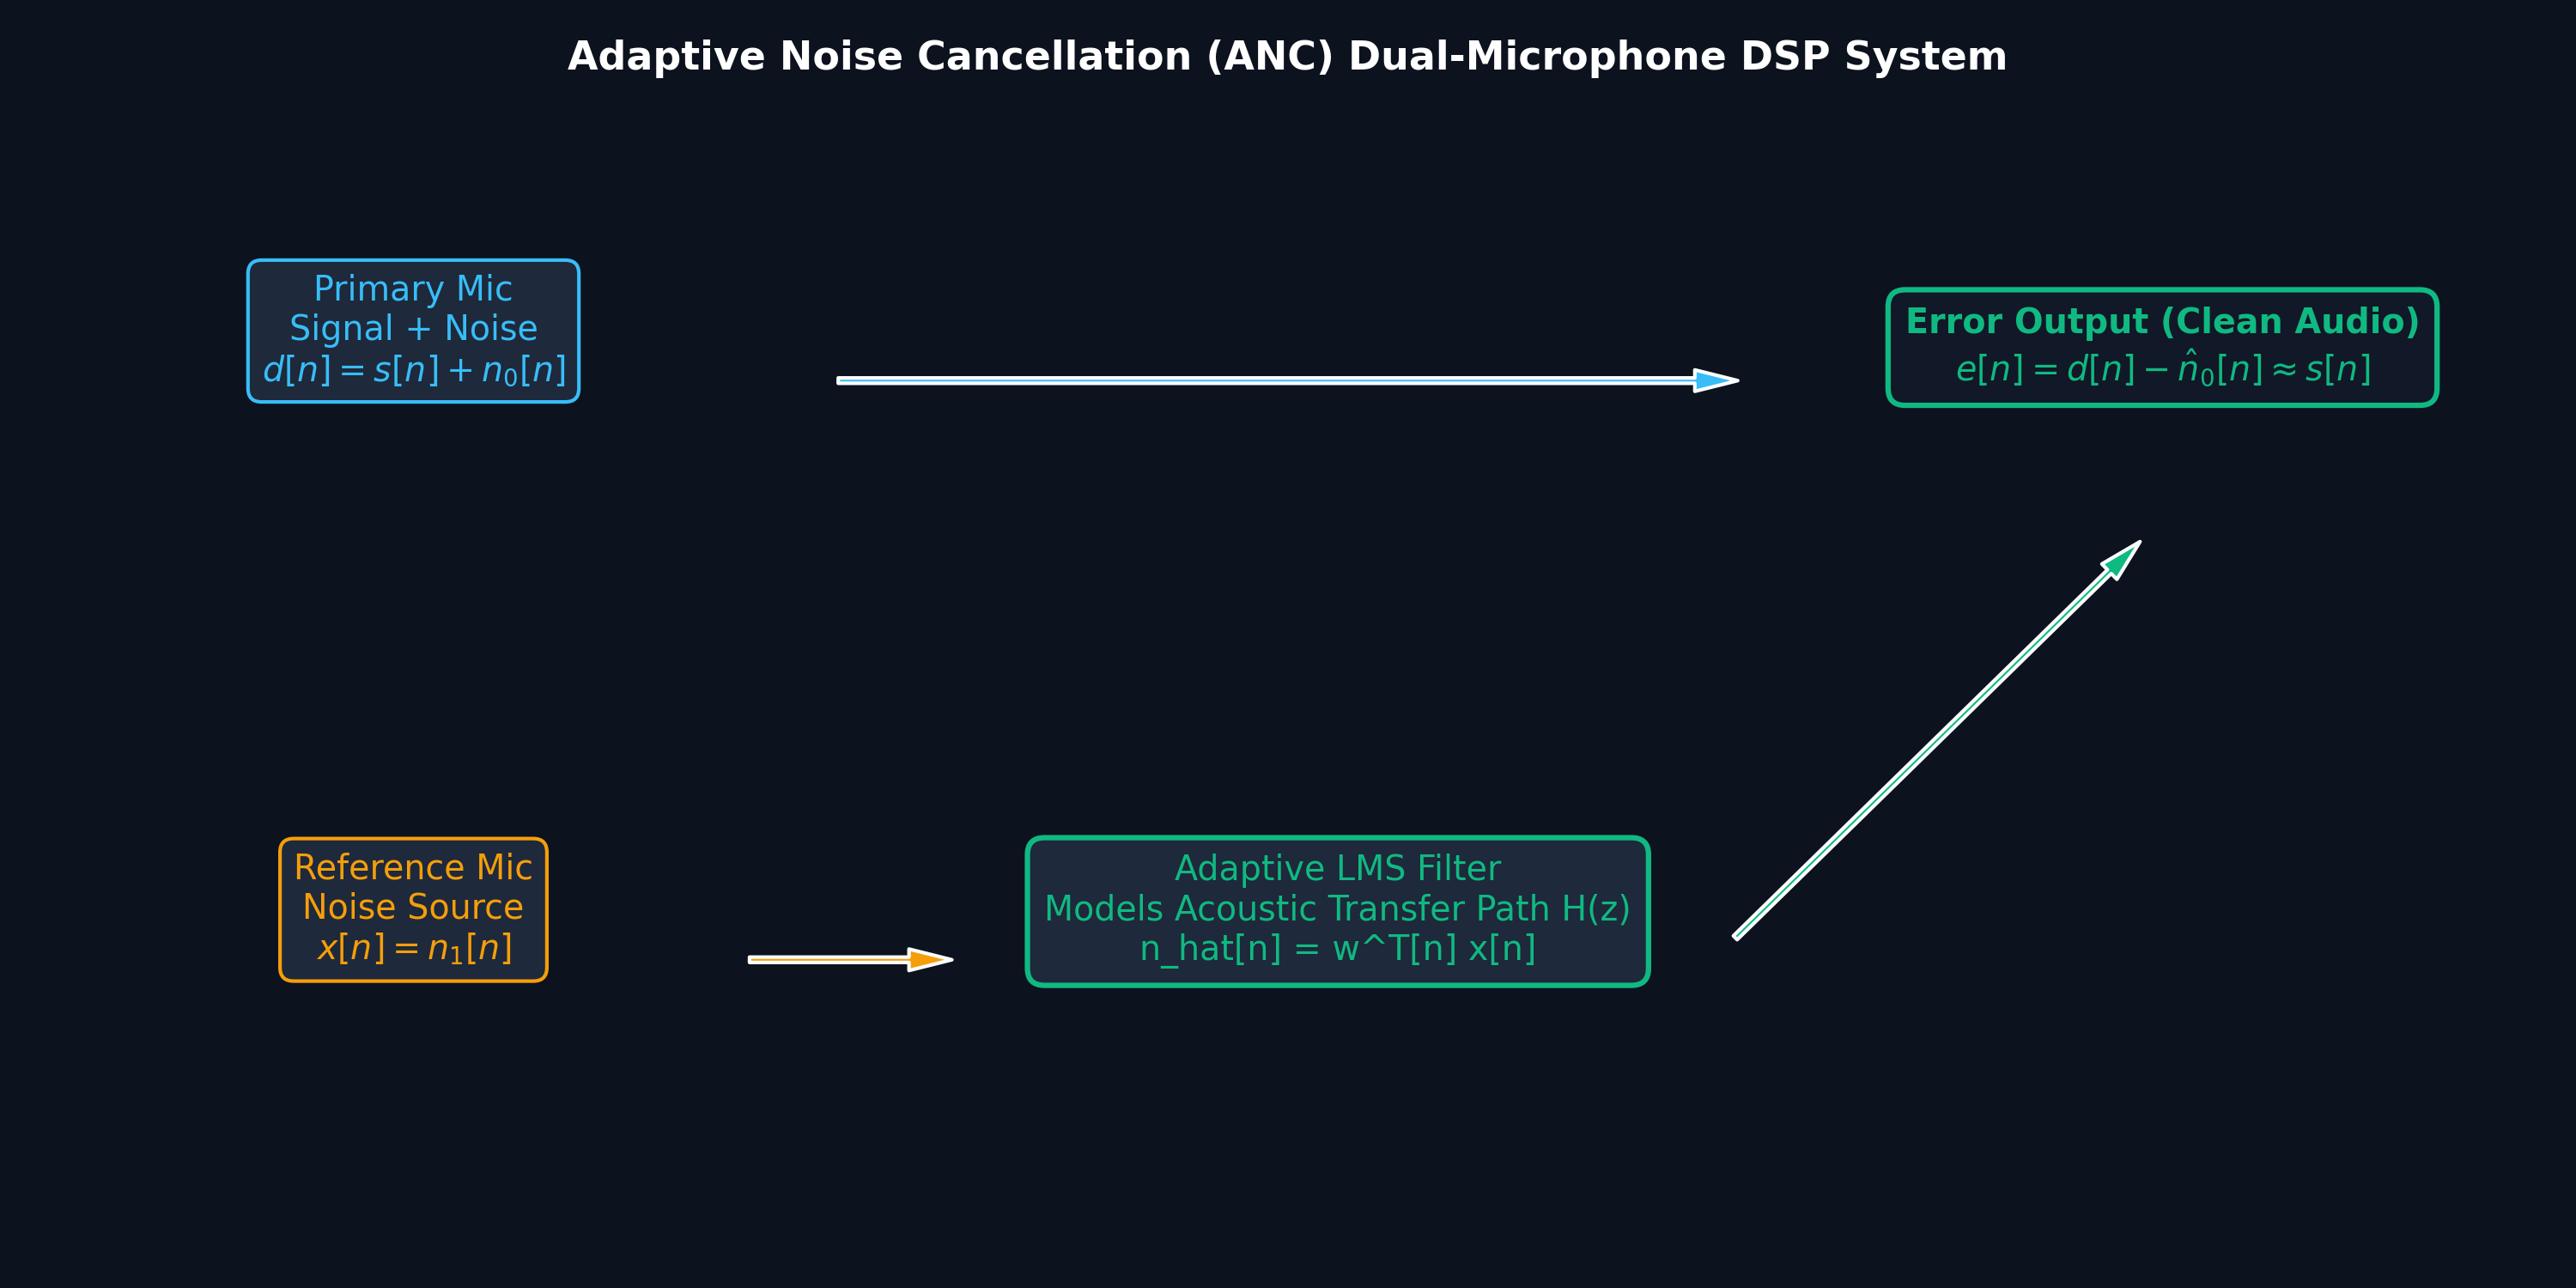
\includegraphics[width=0.85\textwidth]{images/adaptive_noise_cancellation_system.png}
    \caption{Acoustic Adaptive Noise Cancellation (ANC) System Architecture using LMS Error Minimization.}
\end{figure}

\begin{figure}[H]
    \centering
    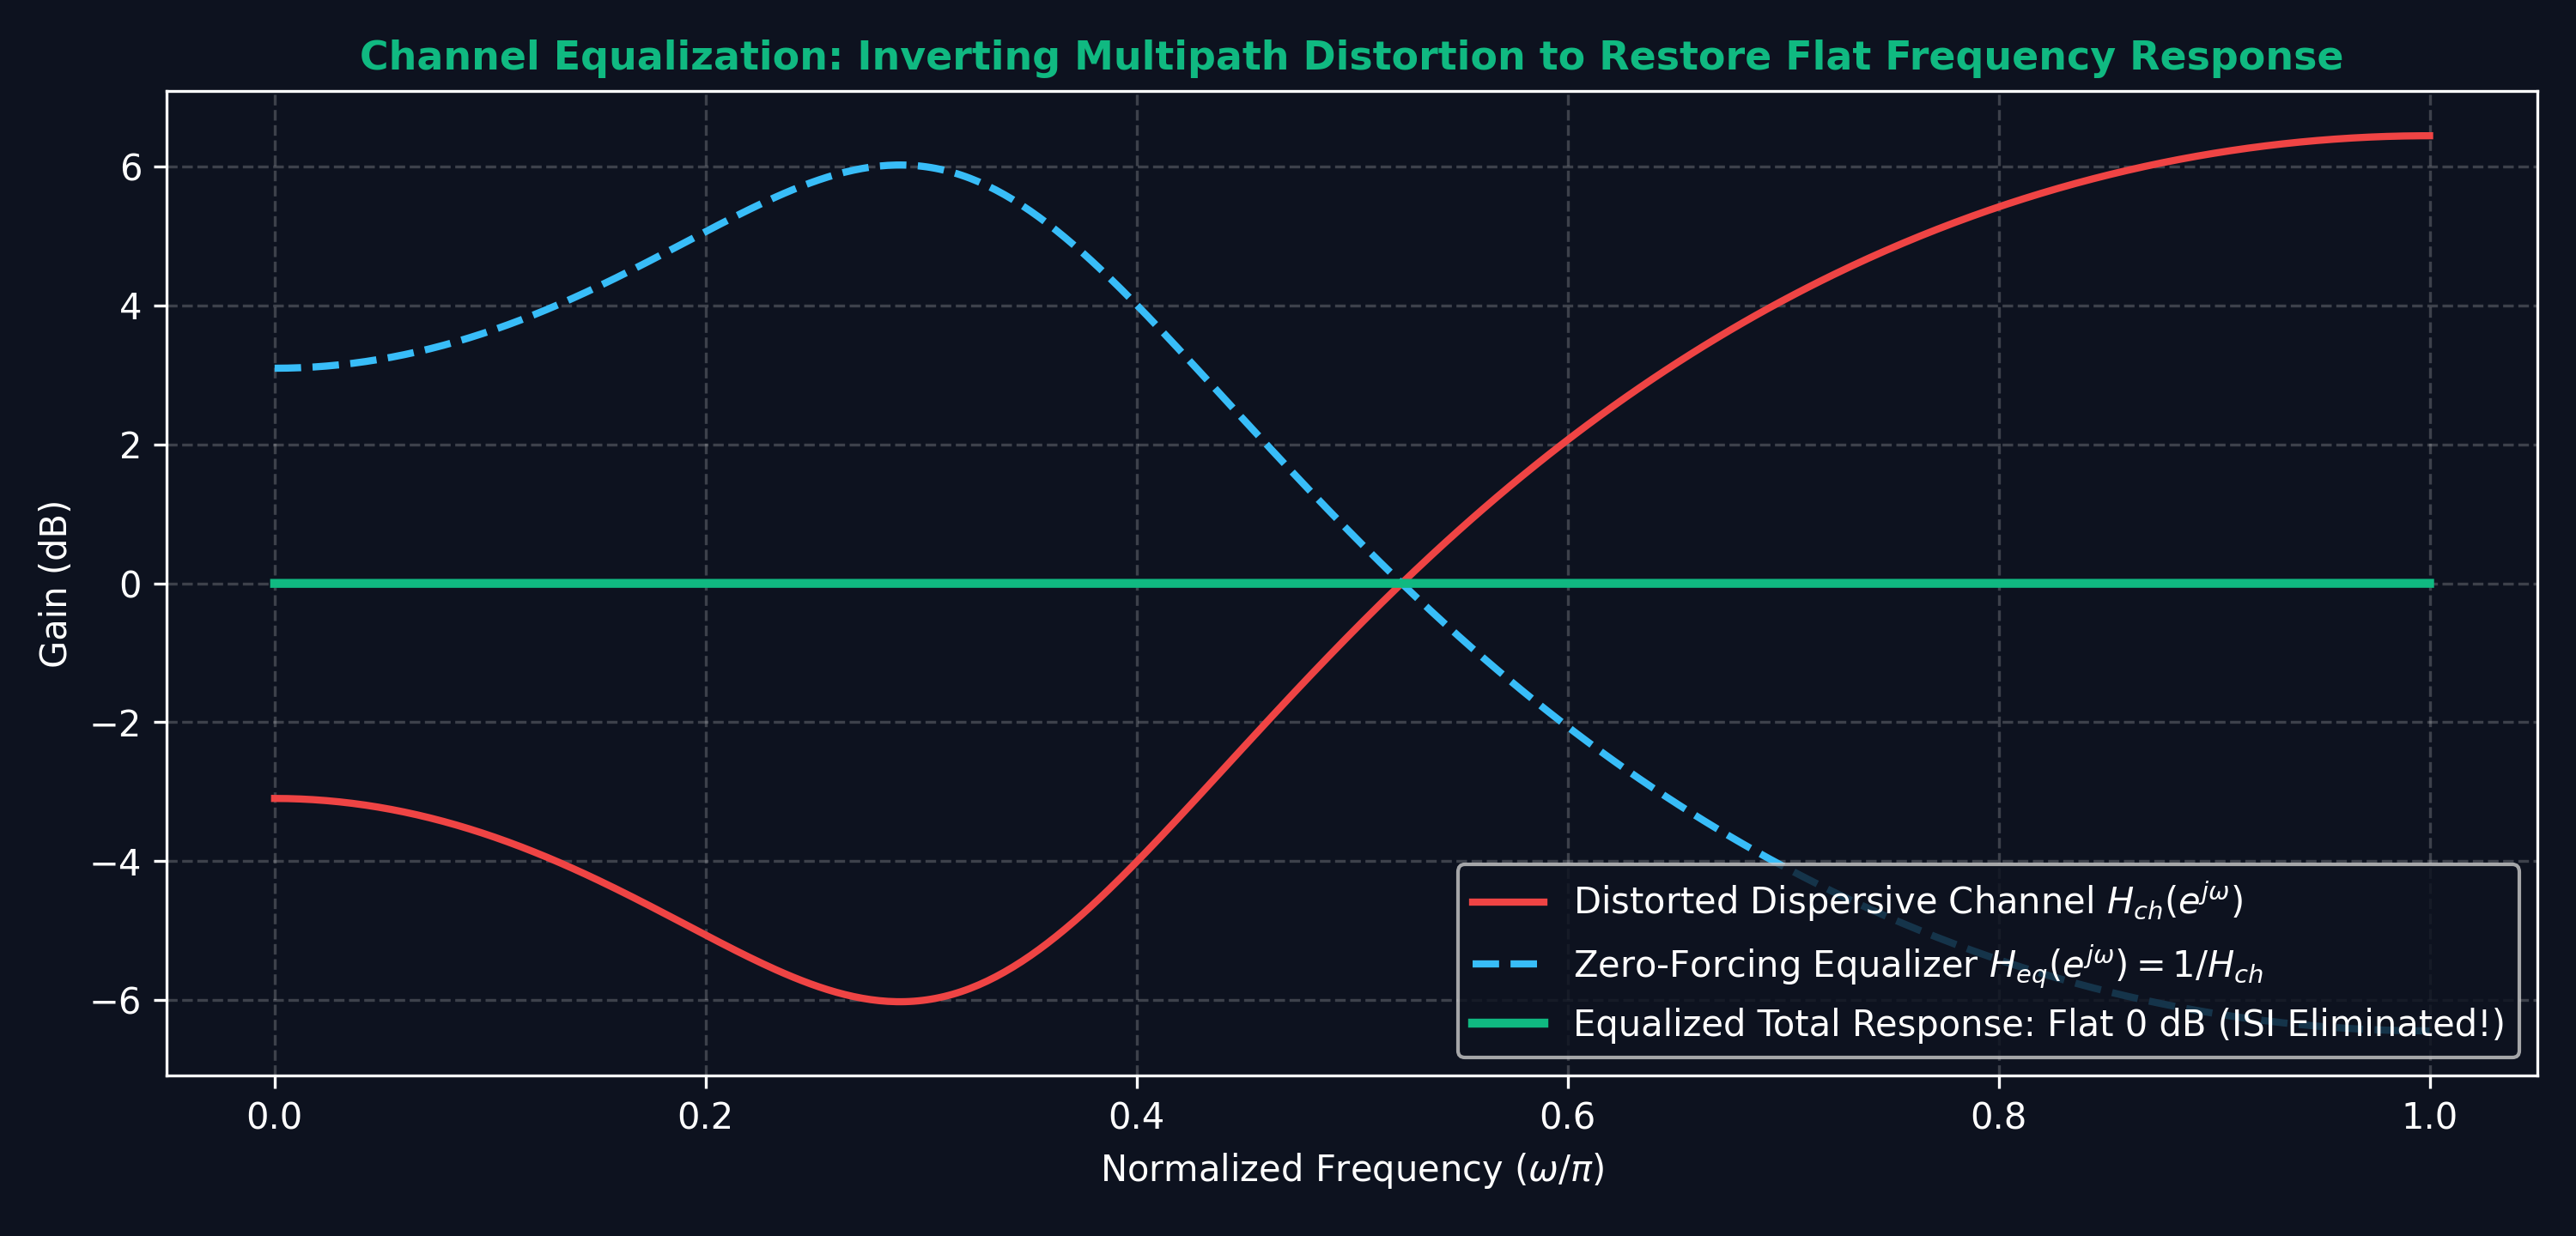
\includegraphics[width=0.85\textwidth]{images/channel_equalizer_frequency_response.png}
    \caption{Multipath Channel Equalization: Inverting Frequency Distortion to Restore Flat Transfer Function.}
\end{figure}


Designing a DSP system requires traversing from abstract mathematics to physical hardware.

\subsection{Requirements Analysis}
Before writing any code, engineers must define:
1. \textbf{Sampling Rate ($f_s$):} Dictates the computational budget.
2. \textbf{Dynamic Range \& SNR:} Determines the word length.
3. \textbf{Latency:} Critical for real-time control loops.
4. \textbf{Power Consumption:} Dictates hardware selection.

\subsection{Algorithm Selection}
\textbf{FIR vs. IIR:} FIR provides linear phase and unconditional stability but requires more MAC operations. IIR requires fewer coefficients but is prone to limit cycles.

\subsection{Floating-Point vs. Fixed-Point}
Floating-point is easier to program with vast dynamic range but takes more power/area. Fixed-point is harder to program (requires manual scaling) but offers low power and high speed.

\section{Fixed-Point DSP Implementation}

\subsection{Two's Complement Arithmetic}
Most DSPs use two's complement. An $N$-bit number represents values from $-2^{N-1}$ to $2^{N-1}-1$.

\subsection{Q-Format Notation}
To represent fractional numbers in integer hardware, we use $Q(m.n)$ notation:
\begin{itemize}
    \item $m$: Number of integer bits (including sign bit).
    \item $n$: Number of fractional bits.
    \item Total bits: $N = m + n$.
    \item Range: $[-2^{m-1}, 2^{m-1} - 2^{-n}]$
\end{itemize}

\subsection{Overflow Handling}
When additions exceed the maximum value, two's complement wraps around. \textbf{Saturation Arithmetic} clamps the result to the maximum/minimum representable value instead of wrapping.

\subsection{Scaling and Rounding}
When multiplying two $Q(m.n)$ numbers, the result is in $Q(2m.2n)$. To store this back, we must shift right by $n$ bits and round. Truncation causes a negative DC bias. Rounding (adding $2^{n-1}$ before truncating) provides zero-mean error.

\subsection{Block Floating-Point}
A block of data shares a single exponent. The block is scanned for the maximum magnitude, and all values are scaled to maximize dynamic range.

\section{DSP Processor Architecture}
\subsection{Harvard Architecture}
Separate memory spaces and buses for instructions and data. Allows the processor to fetch an instruction and read/write data simultaneously.

\subsection{Single-Cycle MAC}
The Multiply-Accumulate operation executes in a single cycle using a dedicated hardware multiplier and a wide accumulator.

\subsection{Barrel Shifter}
Can shift a data word left or right by any number of bits in a single clock cycle. Crucial for scaling.

\subsection{Circular Buffers}
FIR filters use a delay line. A circular buffer updates pointers modulo the buffer size, implementing delays with zero data-movement overhead.

\subsection{SIMD Extensions}
Single Instruction, Multiple Data allows one instruction to operate on multiple data points simultaneously.

\section{FPGA vs DSP Processor vs GPU}
\begin{table}[H]
\centering
\begin{tabular}{@{}llll@{}}
\toprule
\textbf{Feature} & \textbf{FPGA} & \textbf{DSP Processor} & \textbf{GPU} \\ \midrule
\textbf{Architecture} & Reconfigurable logic & Programmable CPU & Massive SIMD \\
\textbf{Parallelism} & True hardware & Instruction level & Thread-level \\
\textbf{Latency} & Extremely low & Low & High \\
\textbf{Power Eff.} & Very high & High & Low \\
\bottomrule
\end{tabular}
\caption{Hardware Trade-offs}
\end{table}

\section{Real-Time System Design}
\subsection{Interrupt vs DMA}
\textbf{DMA (Direct Memory Access):} Hardware writes ADC samples directly to memory. CPU is only interrupted when a full block is ready.

\subsection{Double-Buffering (Ping-Pong)}
While the CPU processes Buffer A, the DMA fills Buffer B. Hides I/O latency.

\subsection{Worst-Case Execution Time (WCET)}
The WCET must be strictly less than the block processing deadline.

\section{Course Review --- Key Connections}

\section{Emerging Trends \& Career Paths}
\textbf{Trends:} Deep Learning on Edge (TinyML), Neuromorphic Computing, Quantum Signal Processing, Software-Defined Radio. \\
\textbf{Careers:} RF/Communications, Embedded Audio/Video, Power Electronics, Biomedical, Autonomous Vehicles.

\section{Comprehensive Final Exam Problems}

\textbf{Problem 1: Filter Design \& Quantization} \\
Design a 1st-order IIR lowpass filter with a pole at $z = 0.8$. Implement it in $Q(2.14)$. \\
\textit{Solution:} Difference equation is $y[n] = x[n] + 0.8 y[n-1]$. $0.8 \times 2^{14} \approx 13107$. Truncation error variance $\sigma_e^2 = \frac{(2^{-14})^2}{12} \approx 3.1 \times 10^{-10}$. Output noise variance $\sigma_y^2 = \sigma_e^2 \frac{1}{1 - 0.8^2} = 8.6 \times 10^{-10}$.

\textbf{Problem 2: Adaptive Filtering} \\
An LMS filter with $M=2$ taps. Input $x[n]$ is white noise with variance 1. Find max step size $\mu$. \\
\textit{Solution:} $\mathbf{R} = \mathbf{I}$. $\text{Tr}(\mathbf{R}) = 2$. Stability condition $0 < \mu < \frac{1}{\text{Tr}(\mathbf{R})} \implies 0 < \mu < 0.5$.

\textbf{Problem 3: Multirate System Design} \\
Upsample $8\text{ kHz}$ to $48\text{ kHz}$. \\
\textit{Solution:} Interpolation factor $L=6$. Insert 5 zeros. Design lowpass $H(z)$ with cutoff $\pi/6$. Decompose into 6 polyphase components to compute efficiently at $8\text{ kHz}$.

\section{Key Formulas Summary}
\begin{table}[H]
\centering
\begin{tabular}{@{}ll@{}}
\toprule
\textbf{Concept} & \textbf{Formula} \\ \midrule
Q-format Range & $[-2^{m-1}, 2^{m-1} - 2^{-n}]$ \\
LMS Update & $\mathbf{w}[n+1] = \mathbf{w}[n] + 2\mu e[n]\mathbf{x}[n]$ \\
LMS Stability & $0 < \mu < \frac{1}{\text{Tr}(\mathbf{R})}$ \\
Zero-Forcing & $E(z) = \frac{1}{C(z)}$ \\
Polyphase Filter & $H(z) = \sum_{k=0}^{L-1} z^{-k} E_k(z^L)$ \\
\bottomrule
\end{tabular}
\caption{Key Formulas}
\end{table}

\section{Checkpoint Questions}
\begin{enumerate}
    \item \textbf{Q1:} Why is a barrel shifter essential in a fixed-point DSP processor? \\
    \textit{Answer:} Multiplying $Q(m.n)$ numbers gives a $Q(2m.2n)$ product. To store it back, we shift right by $n$ bits. A barrel shifter does this in one cycle.
    
    \item \textbf{Q2:} Compare truncation vs rounding. \\
    \textit{Answer:} Truncation discards lower bits, introducing a negative DC bias. Rounding adds $2^{n-1}$ before truncating, providing a zero-mean error.
    
    \item \textbf{Q3:} How does double-buffering prevent data loss? \\
    \textit{Answer:} DMA fills Buffer A while CPU processes Buffer B. They swap roles when Buffer A is full, decoupling continuous I/O from bursty CPU processing.
\end{enumerate}

\end{document}
